\section{Sets}
\index{Set}
\epigraph{A pack of wolves, a bunch of grapes, or a flock of
pigeons are all examples of sets of things.
The mathematical concept of a set can be used as the foundation
for all known mathematics.
The purpose of this little book is to develop the basic properties
of sets.\\
\ldots \\
One thing that this development will not include is a definition
of sets.
The situation is analogous to the familiar axiomatic approach to
elementary geometry.
That approach does not offer a definition of points and lines;
instead it describes what it is that one can do with those
objects.
The semi-axiomatic point of view adopted here assumes that the
reader has the ordinary, human, intuitive (and frequently
erroneous) understanding of what sets are; the purpose of the
exposition is to delineate some of the things one can correctly do
with them.}%
{Halmos, \textit{Naive Set Theory}\cite{Halmos1960Naive}}

\vfill

\emph{Sets} are a foundation for everything we are going to do,
but they turn out to be surprisingly hard to define precisely,
from first principles, without introducing paradoxes.

\vfill

\label{sec:math-sets}
\lstset{language=Clojure}

\subsection{Defining sets}
\epigraph{All the basic principles of set theory, except only the
axiom of extension, are designed to make new sets out of old ones.
The first and most important of these basic principles of set
manufacture says, roughly speaking, that anything intelligent one
can assert about the elements of a set specifies a subset, namely,
the subset of those elements about which the assertion is true.}
{Halmos,
\textit{Naive Set Theory}, section 2~\cite{Halmos1960Naive}}

\begin{description}

\item[Specification]

A \gls{Set}, at its most fundamental, is a defined by a rule,
or method,
for determining if any given 'thing' is an element: 
$s \glssymbol{elementOf} \aSet{S}$.
\footnote{$(s \notin \aSet{S}) = \text{not}(s \in \aSet{S})$.}
($s \not\in \aSet{S}$)
%, or in pseudocode:
%\lstinline|(element-of $\aSet{S}$ $s$)|.
An example, in standard set notation:
the even numbers $= \{ i | \, i/2 \, \text{is an integer}\}$.

\item[Enumeration]

However, it's difficult to do much interesting with a set
unless we have some way of finding, or generating elements.
So another common way to specify a set is by enumeration:
For example, the even numbers $= \{ \ldots, -4, -2, 0, 2 ,4,
\ldots \}$.

The enumeration notation above is something of a cheat ---
although it's straightforward enough for finite sets, it relies on
the reader correctly recognizing the implied pattern for countable
sets.
And it fails for uncountable sets like the real numbers.

\end{description}

What's unstated, but required, in both these approaches, is the
existence of some prior 'universe' set, $\aSet{U}$, and a function
(see~\autoref{sec:Functions}) we can apply to the elements of
$\aSet{U}$ to determine the set of interest:

\begin{description}
\item[Specification] 
$\aSet{S} =
\{ u \glssymbol{elementOf} \aSet{U} | p(u) = \text{true} \}$ 

For example: the even numbers $= \{ i \glssymbol{elementOf} 
\glssymbol{Integers} |
 \, i/2 \glssymbol{elementOf} \glssymbol{Integers} \}$.

\item[Enumeration]
$\aSet{S} =
\{ f(u) | u \glssymbol{elementOf} \aSet{U} \}$ 

For example: the even numbers $= \{ 2*i | \, i
\glssymbol{elementOf} \glssymbol{Integers} \}$.

\end{description}
A variation on 
``turtles all the way down''~\cite{xkcd:Turtles, wiki:Turtles},
this approach may be a bit unsatisfying.
It does, however, have the advantage of preventing self-reference
paradoxes (for example, 
the set of all sets that do not contain themselves); 
see~\cite[Halmos, \textit{Naive Set Theory,} section 2]
{Halmos1960Naive} for details.

% \gls{empty set}
One set that doesn't require any turtles is 
the empty set, $\varnothing$.


Both approaches raise the fascinating issue of 
computability/decidability~\cite{church1936unsolvable,
turing1936computability,
turing1938computable-correction,
turing1937computability-lambda},
which I am going to pass over here, except to note the 
'halting problem'~\cite{wiki:Halting-problem}:

If we call $p(u)$ to determine if $u \in \aSet{S}$, 
it might return $\text{true}$, might return $\text{false}$,
or it might not return at all.
In the third case, we might define $u \in \aSet{S}$ as only those
$u$ where $p(u)$ halts and returns $\text{true}$, but it turns 
out that given $p$ and $u$, deciding whether $p(u)$ will ever
finish is itself undecidable (more turtles \ldots).

The practical version of this is that, even in cases where we
might be able to determine that $p(u)$ that will eventually halt
and return something, we might not be able to afford to wait that
long.
Pragmatically, we will have to restrict ourselves to sets where we
can guarantee an answer fast enough for the context in which the
sets are being used.

\subsubsection{Cardinality}

% \gls{cardinality}  \gls{countable infinity} \gls{uncountable
% infinity} \gls{cardinal numbers}
The cardinality of a set in the number of elements.
For our purposes, the possibilities that matter are \emph{finite,}
\emph{countably infinite}, the cardinality of the
\gls{NaturalNumbers}, $\aleph_{0}$, or \emph{uncountably
infinite}, which means the set has more elements than the
\gls{NaturalNumbers}.
(I'm ignoring the distinction between different uncountable
infinities.
See~\cite{wiki:cardinal-number} for an introduction to the other
possibilities.)

Notation for set cardinality varies widely:
$\#\aSet{S}$,  $|\aSet{S}|$,
$\bar{\bar{\aSet{S}}}$, $n(\aSet{S})$,
$\text{card}(\aSet{S})$, \ldots, nearly all of which conflict
with something (eg $\#\{ 0 \, 1 \, 2 \} = 3$ vs 
\lstinline|#{1 2 3}| Clojure set syntax).
I will use $\text{cardinality}(\aSet{S})$.

 
\subsubsection{Identity}

The question of whether two sets are the same set is a recurring
locus of ambiguity in mathematics.

One issue is the difference between the 'set' and the 
'set definition', which is rarely made clear.

Halmos~\cite{Halmos1960Naive} starts with the \emph{Axiom of
extension:} two sets are the \emph{same thing} if they have the
same elements (regardless of how they are defined).

Example: 
$\{ 2*i | \, i \in \glssymbol{Integers} \}$
and
$\{ i \in \glssymbol{Integers} |
 \, i/2 \in \glssymbol{Integers} \}$
are two distinct definitions of the same set. 
 
Pragmatically, however, it's going to be much easier to determine
if two set definitions are the same, than determining if two
different definitions generate the same elements, which would,
after all, be undecidable in general.

Another source of ambiguity is a common tendency to blur the 
distinction between sets whose elements are related by some natural
identity. 

Example: we can define the rational numbers as (equivalence
classes of) pairs of integers:
$\glssymbol{RationalNumbers} = \glsdesc{RationalNumbers}$.
Strictly speaking, the rational number $i/1$ is a different thing
from the integer $i$, but it's nearly universal to identify the
subset of the rationals with denominator $1$ with the integers and
take $\glssymbol{Integers} \subset \glssymbol{RationalNumbers}$.

\subsubsection{Subsets, partitions, and quotients}

Families: $\{ \aSet{S}_{i} | i \in \, \text{index set} \, \aSet{I}
\}$.


%\gls{subset} \gls{superset}

$\aSet{A} \subseteq \aSet{B}$ ($\aSet{B} \supseteq \aSet{A}$)
means
every element of $\aSet{A}$ is an element of $\aSet{B}$, 
that is, $a \in \aSet{A}$ 
implies $a \in \aSet{B}$.
I reserve $\aSet{A} \subset \aSet{B}$ (($\aSet{B} \supset
\aSet{A}$)) for strict subsets;
it means $\aSet{A} \subseteq \aSet{B}$
and there is some $\b\in\aSet{B}$ which
is not in $\aSet{A}$.


%\gls{power set}

The \emph{power set}, ${\displaystyle \wp}(\aSet{S})$ is the set 
of all subsets of
$\aSet{S}$.

%\gls{intersection} \gls{union} \gls{set-difference}
As usual, $\aSet{A} \cap \aSet{B}$ is the set of elements in both 
$\aSet{A}$ and $\aSet{B}$; $\aSet{A} \cup \aSet{B}$ are those things
that are in either $\aSet{A}$ or $\aSet{B}$.

$\aSet{A} \cap \aSet{B} \cap \aSet{C} 
= (\aSet{A} \cap \aSet{B}) \cap \aSet{C} 
= \aSet{A} \cap (\aSet{B} \cap \aSet{C}) $

$\bigcap_{i \in \aSet{I}} \aSet{S}_{i} = \{ s | s \in \aSet{S}_{i}
\forall \aSet{S}_{i} \}$

$\aSet{A} \setminus \aSet{B}$ are the elements of $\aSet{A}$ 
not in $\aSet{B}$.

%\gls{partition}
A partition of $\aSet{S}$ is a set of disjoint nonempty subsets of
$\aSet{S}$ whose union is $\aSet{S}$.

\subsubsection{Cartesian products}

% \gls{tuple}
A tuple is a fixed length list, which I will write, for example,
$[a \, b \, c]$, in a Clojure-like syntax,
or sometimes as $a \times b \times c$.

% \gls{cartesian-product}
The cartesian product set 
$\aSet{A} \times \aSet{B} =
\{[a \, b] | a \in \aSet{A} \text{ and } b \in \aSet{B}\}$.

Extending this notation beyond two terms,
$\aSet{A} \times \aSet{B} \times \aSet{C}$,
introduces ambiguity typically ignored in mathematics literature,
using the implied natural identity mentioned above.
Strictly speaking,
\begin{itemize}
  \item $\aSet{A} \times \aSet{B} \times \aSet{C} = 
  \{[a \, b \, c] | \ldots \}$
  \item $\aSet{A} \times (\aSet{B} \times \aSet{C}) = 
  \{[a \, [b \,c]] | \ldots \}$
  \item $(\aSet{A} \times \aSet{B}) \times \aSet{C} = 
  \{[[a \, b] \, c]] | \ldots \}$
\end{itemize}
are 3 distinct sets.

\subsection{computation}

\subsubsection{Java}
\lstset{language=Java}

Java provides an interface \lstinline|java.util.Set| intended for
possibly mutable, finite sets (\autoref{java.util.Set:general},
 \autoref{java.util.Set:countable}, 
 \autoref{java.util.Set:finite}, 
 and
\autoref{java.util.Set:optional}).

%-----------------------------------------------------------------
\begin{lstlisting}[
 caption={[\texttt{java.util.Set} general]\texttt{java.util.Set} 
 operations applicable to any set.}, 
 label=java.util.Set:general]
boolean contains (Object o) //$ \; o \in \aSet{S}$
boolean containsAll (Collection c) //$\;\aSet{C}\subseteq\aSet{S}$ 
boolean isEmpty () //$ \; \aSet{S} = \varnothing $
boolean equals (Object o) //$\; \aSet{S} = \aSet{O} $
\end{lstlisting}
%-----------------------------------------------------------------
\begin{lstlisting}[
 caption={[\texttt{java.util.Set} countable]\texttt{java.util.Set} 
 operations requiring countable sets. Note, however, that 
 iterators that never end will cause havoc with almost all Java
 code}, 
 label=java.util.Set:countable]
Iterator iterator ()
Spliterator spliterator ()
\end{lstlisting}
%-----------------------------------------------------------------
\begin{lstlisting}[
 caption={[\texttt{java.util.Set} finite]\texttt{java.util.Set} 
 operations requiring finite sets. Note that changing to
 \texttt{size()} to be Object valued would enable representing sets
 of arbitrary cardinality.}, 
 label=java.util.Set:finite] 
int size () 
Object[] toArray ()
Object[] toArray (Object[] a)
\end{lstlisting}
%-----------------------------------------------------------------
\begin{lstlisting}[
 caption={[\texttt{java.util.Set}]\texttt{java.util.Set} optional
 operations, requiring mutable sets.}, 
 label=java.util.Set:optional,]
boolean add(E e) //$\; \aSet{S} \leftarrow \aSet{S} \cup \{e\} $
boolean addAll(Collection c) //$\;\aSet{S}\leftarrow\aSet{S}\cup\aSet{C}$ 
void  clear() //$\; \aSet{S} \leftarrow \varnothing $ 
boolean remove (Object o) //$\;\aSet{S}\leftarrow\aSet{S}\setminus\{e\}$
boolean removeAll (Collection c) //$\;\aSet{S}\leftarrow\aSet{S}\setminus\aSet{C}$ 
boolean retainAll (Collection c) //$\;\aSet{S}\leftarrow\aSet{S}\cap\aSet{C}$
\end{lstlisting}
%-----------------------------------------------------------------

More Java set classes? Guava or Apache Commons?
Set operations, union, cartesian products, \ldots.

\subsubsection{Clojure}
\lstset{language=Clojure}

Idiomatic Clojure sets are immutable, although it provides easy
access to any mutable or immutable Java implementation of
\lstinline|java.util.Set|.

Clojure provides an (unfortunate) literal syntax for finite
enumerated sets: 
\lstinline|#{0 1 2}|, and 4 ways to create sets:
\begin{description}
\item[\texttt{hash-set}] A function equivalent to the
literal syntax \lstinline|#{}|
\item[\texttt{sorted-set}/\texttt{sorted-set-by}] Returns
sets that iterate over their elements in their natural order (in the
order of the supplied comparator). Like Java sorted collections,
can't handle partial orderings.
\item[\texttt{set}] Coerce any collection into a set.
\item[\texttt{into}] A general way to coerce any collection
into another type.
\end{description}

Idiomatic Clojure provides an informally specified functional
'API' for finite sets. Most of these functions do will something
for all Clojure collections, not always what you would expect:
\begin{lstlisting}[
 caption={Clojure set 'API'}, 
 label=Clojure:set-API,]
(contains? s x) ;;  $x \in \aSet{S}$.
(empty? s) ;; $\aSet{S} = \varnothing$
(count s) ;; $\text{cardinality}(\aSet{S})$
(conj s x) ;; $\aSet{S} \cup \{x\}$
(disj s x) ;; $\aSet{S} \setminus \{x\}$
(clojure.set/intersection s0 s1 s2 $\ldots$) ;; $\aSet{S}_0 \cap \aSet{S}_1 \cap \aSet{S}_2 \cap \ldots$ 
(clojure.set/union s0 s1 s2 $\ldots$) ;; $\aSet{S}_0 \cup \aSet{S}_1 \cup \aSet{S}_2 \cup \ldots$ 
(clojure.set/difference s0 s1 s2 $\ldots$) ;; $\aSet{S}_0 \setminus (\aSet{S}_1 \cup \aSet{S}_2 \cup \ldots)$
\end{lstlisting}

Confusion with dictionary 'API':
 \lstinline|(s x)| and \lstinline|(get s x)| are similar to
 \lstinline|(contains? s x)| except \lstinline|(contains? s x)| returns
 \lstinline|true| or \lstinline|false|, while the other two return
 \lstinline|x| if \lstinline|x| is in \lstinline|s| \lstinline|nil| otherwise.
The behavior of \lstinline|(s x)| and \lstinline|(get s x)| reflect an
incomplete/inconsistent API treating Clojure collections as
dictionaries (key-value pairs), modeling sets as dictionaries
where the key and value are constrained to be the same.
However, other functions designed for dictionaries (eg
\lstinline|keys|) don't work for sets.
 
\subsubsection{mthcmp}

Set interface:


% \begin{lstlisting}[
% caption={[checksum namespace]Checksum and related functions via
% Java calls}, label=checksum-namespace,]
% (set! *warn-on-reflection* true)
% (set! *unchecked-math* :warn-on-boxed)
% (ns ^{:doc "compute a file checksum."}
%   
%   curate.scripts.checksum
%   
%   (:require [clojure.java.io :as io])
%   (:use [clojure.set :only [difference]])
%   (:gen-class))
% ;;-----------------------------------------------------------------
% (defn checksum [file]
%   (let [input (java.io.FileInputStream. file)
%         digest (java.security.MessageDigest/getInstance "MD5")
%         stream (java.security.DigestInputStream. input digest)
%         bufsize (* 1024 1024)
%         buf (byte-array bufsize)]
% 
%   (while (not= -1 (.read stream buf 0 bufsize)))
%   (apply str (map (partial format "%02x") (.digest digest)))))
% 
% (defn list-dir [dir]
%   (remove #(.isDirectory %)
%           (file-seq (java.io.File. dir))))
% 
% (defn find-dupes [root]
%   (let [files (list-dir root)]
%     (let [summed (zipmap (pmap #(checksum %) files) files)]
%       (difference
%        (into #{} files)
%        (into #{} (vals summed))))))
% 
% (defn remove-dupes [files]
%   (prn "Duplicates files to be removed:")
%   (doseq [f files] (prn (.toString f)))
%   (prn "Delete files? [y/n]:")
%   (if-let [choice (= (read-line) "y")]
%     (doseq [f files] (.delete f))))
% 
% (defn -main [& args]
%   (if (empty? args)
%     (println "Enter a root directory")
%     (remove-dupes (find-dupes (first args))))
%   (System/exit 0))
% \end{lstlisting}
% 
% \lstinputlisting[
% float=htbp,
% caption={[checksum function]Compute a checksum for a file thru Java},
% label=checksum,
% firstline=11,lastline=18]{listings/checksum.clj}
 
\subsection{examples}
 
1d and 2d intervals.
 
% \begin{minipage}{\linewidth}
% \begin{lstlisting}[
% caption={[FileTypeFilter]A file .suffix filter},
% label=FileTypeFilter]
% package img;
% 
% public final class FileTypeFilter 
%   implements java.io.FilenameFilter {
% 
%   private final String _suffix;
% 
%   public final boolean accept (final java.io.File dir,
%                                final String name) {
%     return name.toLowerCase().endsWith(_suffix); }
% 
%   public FileTypeFilter (final String suffix) {
%     super();
%     _suffix = suffix.toLowerCase(); } }
% \end{lstlisting}
% \end{minipage}
% 
% \index{Sets|)}
% 
% \begin{figure}[htbp]
% \centering
% 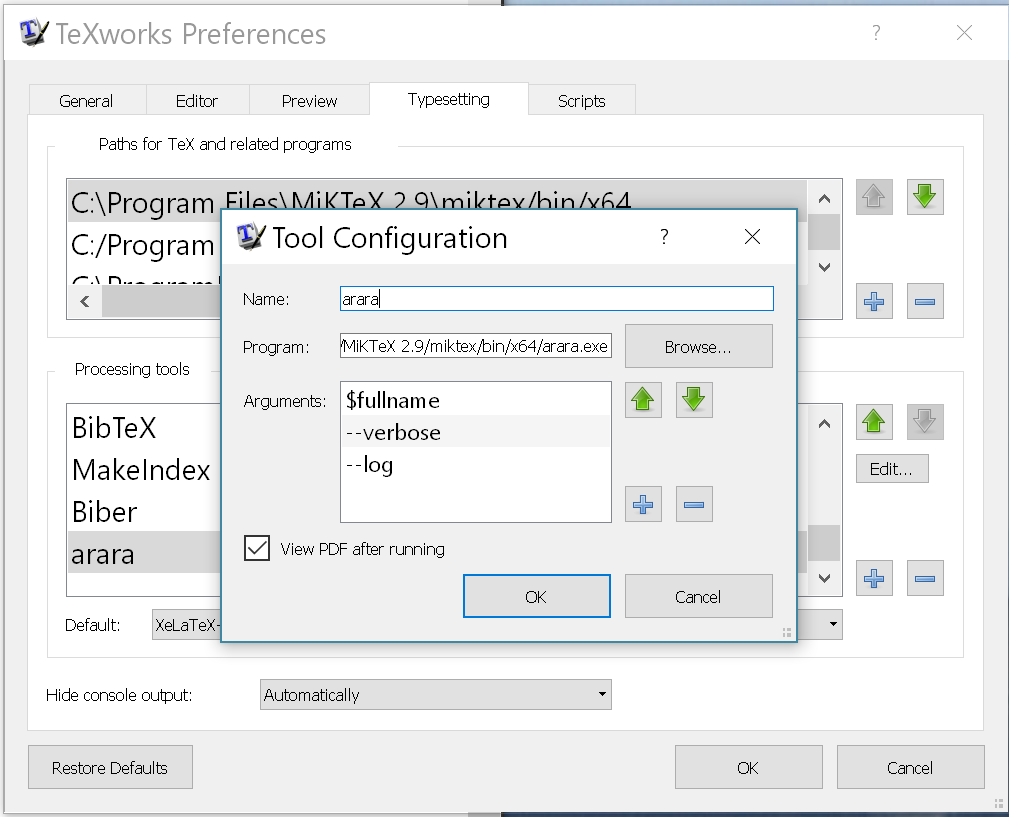
\includegraphics[scale=0.7]{figs/arara.png}
% \caption{Configuring {\TeX}works for \texttt{arara}.}
% \end{figure}
